\chapter{معماری
	O-RAN
}

ساختاری که در 
\lr{O-RAN}
معرفی شده در 
\ref{fig:oran}
قابل مشاهده است. همان‌طور که می‌بینیم علاوه بر قسمت‌هایی که 
\lr{3GPP}
در ناحیه‌ی دسترسی رادیویی تعبیه کرده بود، قسمت‌های جدیدی هم به آن اضافه شده‌اند 

\begin{figure}[H]
	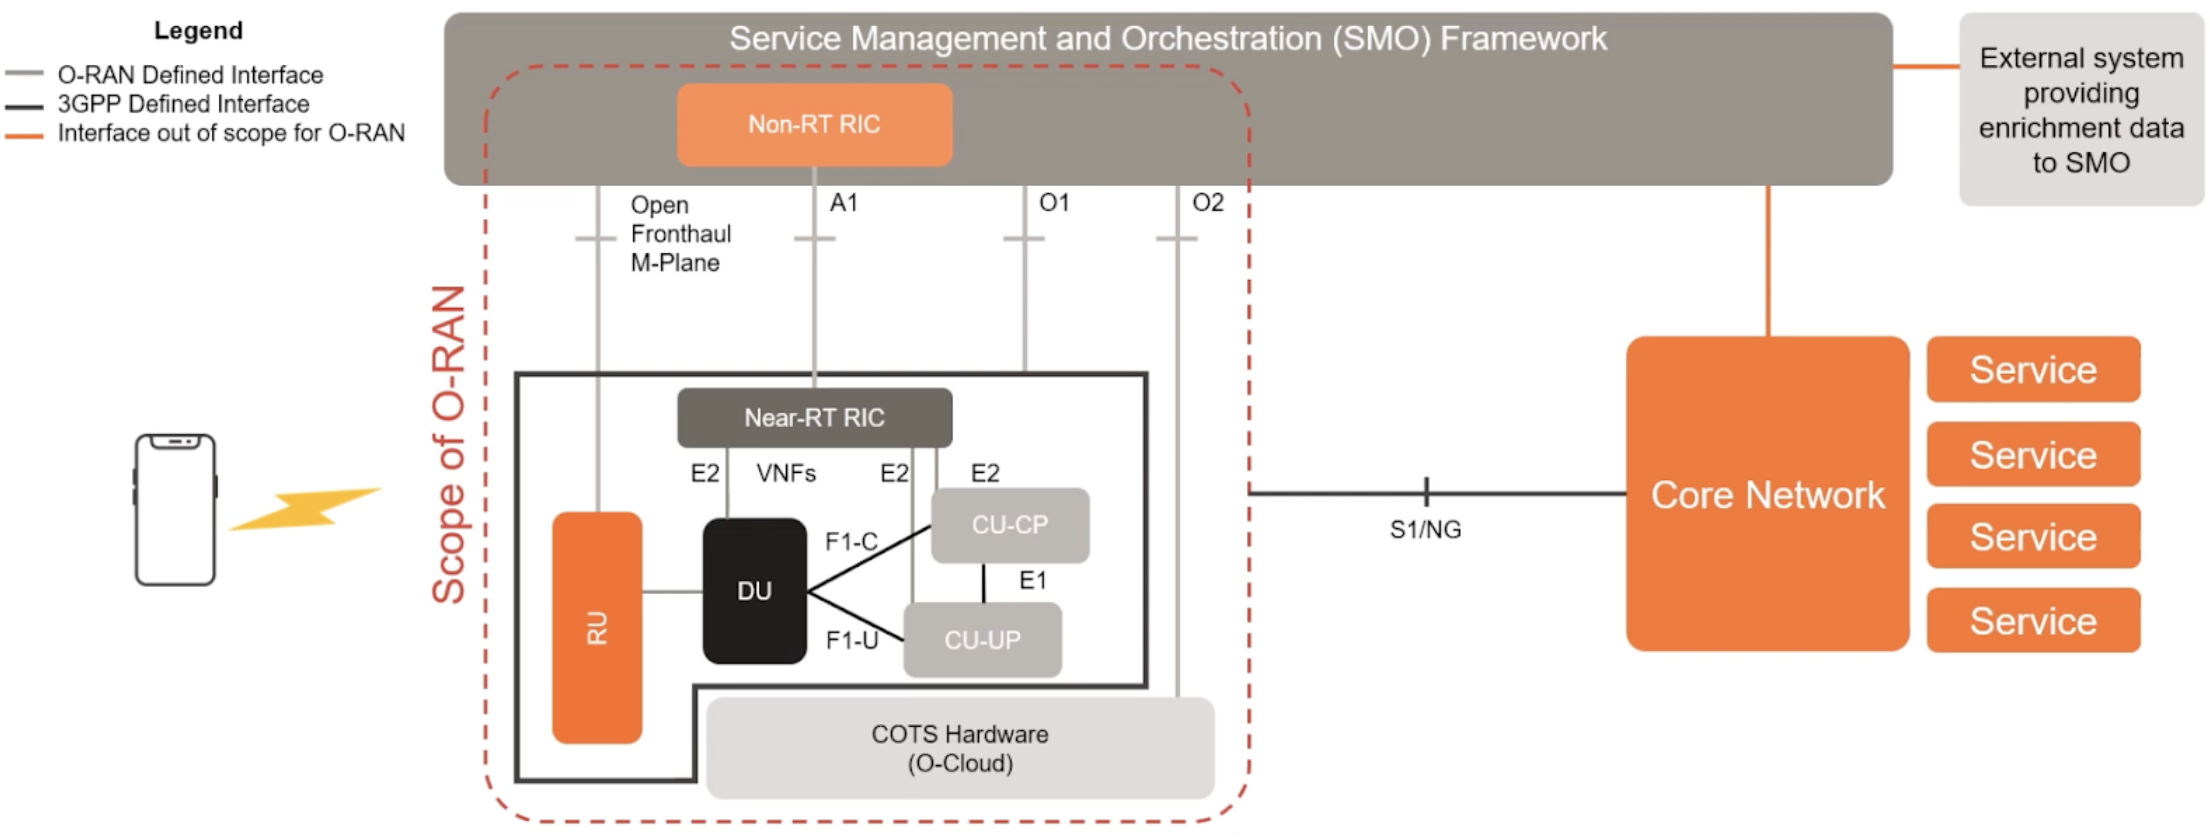
\includegraphics[width=0.85\columnwidth]{Picture/oran.png}
	\centering
	\caption{ساختار کلی شبکه‌های تلفن همراه با
		\lr{O-RAN}}
	\label{fig:oran}
\end{figure}

می‌بینیم که علاوه بر 
\lr{RU}
\lr{DU}،
و 
\lr{CU}،
قسمت‌های جدیدی مانند 
\lr{Near-Real-Time RIC}
و 
\lr{None-Real-Time RIC}
اضافه شده که این قسمت‌های جدید برای کنترل ناحیه‌ی دسترسی رادیویی به صورت هوشمندانه هستند.

در 
\lr{Near-Real-Time RIC}
تمرکز بر کنترل به صورت نزدیک به بلادرنگ است و در 
\lr{None-Real-Time RIC}
کنترل‌های با تاخیر بالاتر از یک ثانیه انجام می‌گیرد. 

یکی از اجزای اصلی
\lr{O-RAN}،
\lr{Near-Real-Time RIC} 
است که وظیفه‌ی کنترل هوشمندانه‌ی ناحیه دسترسی رادیویی با تاخیر نسبتا کم و به صورت نزدیک به بلادرنگ را برعهده دارد.

این قسمت همان‌طور که در 
\ref{fig:nrt-ric0}
هم مشاهده می‌شود، خود از قسمت‌های زیادی تشکیل شده که در اینجا به توضیح آن‌ها نمی‌پردازیم.

\begin{figure}[H]
	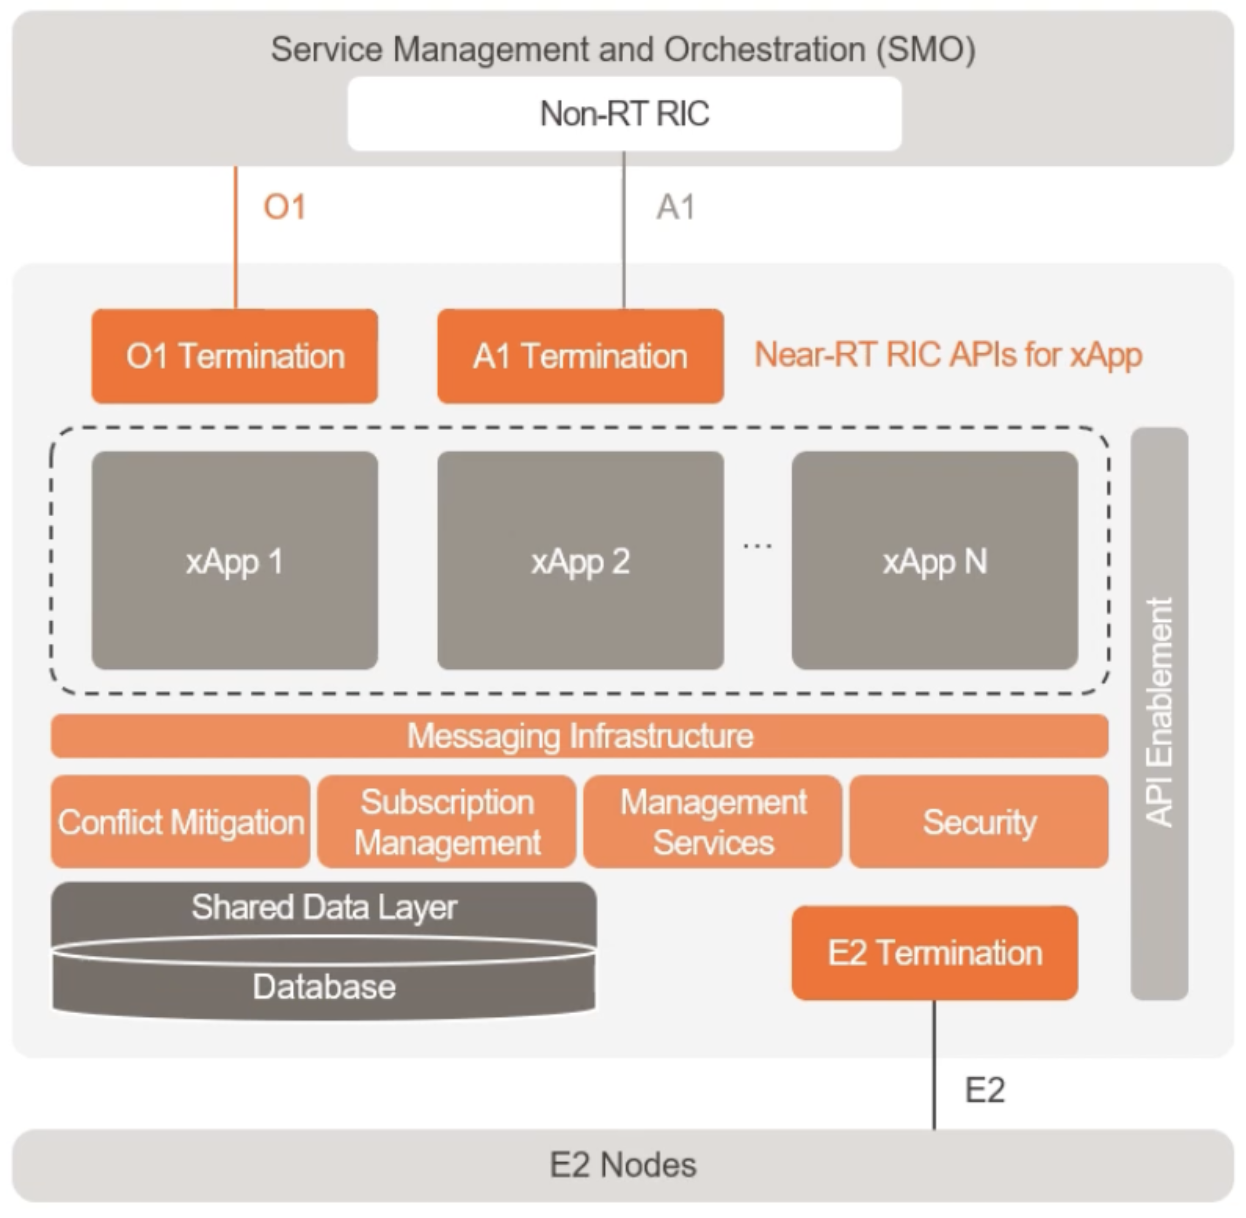
\includegraphics[width=0.85\columnwidth]{Picture/nrt-ric0.png}
	\centering
	\caption{اجزای مختلف موجود در
		\lr{Near-Real-Time RIC}}
	\label{fig:nrt-ric0}
\end{figure}

بخش بعدی‌ای که در 
\lr{O-RAN}
به ناحیه‌ی رادیویی اضافه شده‌است را با این توضیح آغاز می‌کنیم که طبق 
\ref{fig:nonert-ric1}،
قسمت مهم 
\lr{None-Real-Time RIC}
که وظیفه‌ی دادن فرمان‌های کنترلی با تاخیرهای بیش‌تر از یک ثانیه است، خود داخل بخش دیگری به نام
\lr{SMO}
قرار می‌گیرد که خود از قسمت‌های مختلفی تشکیل شده‌است و وظایف گوناگونی را بر عهده دارد.

\begin{figure}[H]
	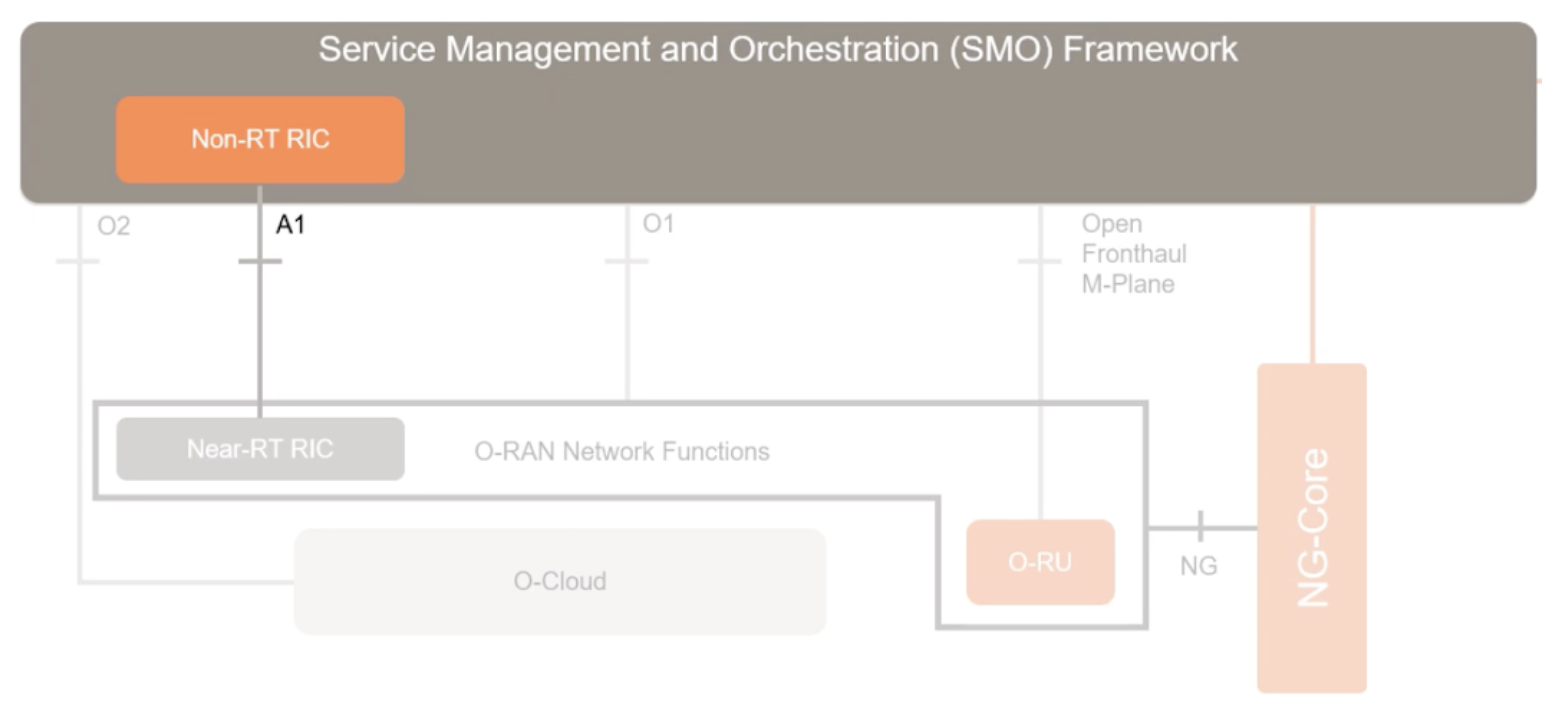
\includegraphics[width=0.85\columnwidth]{Picture/nonert-ric1.png}
	\centering
	\caption{اجزای مختلف موجود در
		\lr{Near-Real-Time RIC}}
	\label{fig:nonert-ric1}
\end{figure}

با توجه به معرفی اجزای جدید در معماری 
\lr{O-RAN}
این نیاز وجود دارد که برای ارتباط بین قسمت‌های مختلف، واسط‌های به صورت استاندارد تعریف شود تا بتوان برنامه‌های مختلفی توسعه داد و اجزای مختلف هم بتوانند به درستی با کمک این واسط‌های استاندارد شده با یک‌دیگر ارتباط برقرار کنند و دیگر همه چیز در اختیار فروشنده‌های قطعات نباشد.

در ادامه واسط‌های مختلفی که در شکل‌های فصل‌های مختلف دیدیم بررسی شده‌اند.

بعضی از این واسط‌ها توسط 
\lr{3GPP}
استاندارد شده‌اند که در 
\ref{fig:int1}
هم آورده شده‌اند. 

واسط
\lr{F1}
برای ارتباط بین
\lr{DU}
و
\lr{CU}
آماده شده است.

واسط
\lr{S1}
برای ارتباط بین
\lr{CU}
و هسته‌ی شبکه معرفی شده است.

در ادامه به بررسی واسط‌های اختصاصی
\lr{O-RAN} 
پرداخته شده.

واسط
\lr{E2}
برای ارتباط بین
\lr{Near-Real-Time RIC}ها
با 
\lr{CU}
و
\lr{DU}
در نظر گرفته شده است.

واسط
\lr{A1}
برای ارتباط بین
\lr{Near-Real-Time RIC}
و 
\lr{None-Real-Time RIC}
معرفی شده است.

واسط
\lr{O1}
برای ارتباط بین
\lr{SMO}
‌و اجزای مختلف اختصاصی 
\lr{O-RAN}
در نظر گرفته شده است.




